\part{Weekly conversation}
\section{2019/7/16}

\begin{enumerate}
  \item 范式:将 PPTL 公式化成规范形式。\\
  $$Q~\equiv~\bigvee_{j=1}^{n_{0}}\left(Q_{ej}~\wedge~\varepsilon\right)~\vee~\bigvee_{i=1}^{n}\left(Q_{ci}~\wedge~\bigcirc~Q_{i}^{\prime}\right)$$

  $Q$,PPTL范式;$Q_p$,原子命题公式;$Q_i^{\prime}$,普通 PPTL 公式。

  \noindent那么PPTL 公式怎么转为范式的四种情况:(最后一种为转为完全范式)。
  \begin{enumerate}[(1)]
    \item PPTL 公式转 $\mathrm{N}_{\mathrm{F}}$。
    \item project 操作转 $\mathrm{N}_{\mathrm{F}}$。
    \item chop 操作转 $\mathrm{N}_{\mathrm{F}}$。
    \item $\mathrm{N}_{\mathrm{F}}$ $\rightarrow$ $C\mathrm{N}_{\mathrm{F}}$\\
    例 $\mathrm{N}_{\mathrm{F}}$ 转 $C\mathrm{N}_{\mathrm{F}}$
    $$\begin{aligned}\left(p \wedge \bigcirc P^{\prime}\right) \vee\left(q \wedge \bigcirc Q^{\prime}\right) \equiv &\left((p \wedge q) \wedge \bigcirc\left(P^{\prime} \vee Q^{\prime}\right)\right) \vee\left((p \wedge \neg q) \wedge \bigcirc P^{\prime}\right) \\ & \vee\left((\neg p \wedge q) \wedge \bigcirc Q^{\prime}\right) \vee((\neg p \wedge \neg q) \wedge \bigcirc f a l s e) \end{aligned}$$

    $$\left(p \wedge \bigcirc P^{\prime}\right) \vee\left(q \wedge \bigcirc Q^{\prime}\right)=false \wedge  \epsilon \vee \left(p \wedge \bigcirc P^{\prime}\right) \vee\left(q \wedge \bigcirc Q^{\prime}\right)$$
  \end{enumerate}
  \item 完全范式(作用:PPTL 完全范式否定简易)

  $$Q~\equiv\left(Q_{e}~\wedge~\varepsilon\right)~\vee~V_{i=1}^{n}\left(Q_{i}~\wedge~\bigcirc~Q_{i}^{\prime}\right)$$

  其中 $\vee_{i}~Q_{i}~\equiv~\text~{~true~and~}~V_{i~\neq~j}\left(Q_{i}~\wedge~Q_{j}\right)~\equiv~false$。

  \item 完全范式的否定\\
  例 $C\mathrm{N}_{\mathrm{F}}$ 的否定
  $$\begin{aligned}\neg \big(\left(p \wedge \bigcirc P^{\prime}\right) \vee\left(q \wedge \bigcirc Q^{\prime}\right)\big) \equiv \neg \Big( &\left((p \wedge q) \wedge \bigcirc\left(P^{\prime} \vee Q^{\prime}\right)\right) \vee\left((p \wedge \neg q) \wedge \bigcirc P^{\prime}\right) \\ & \vee\left((\neg p \wedge q) \wedge \bigcirc Q^{\prime}\right) \vee((\neg p \wedge \neg q) \wedge \bigcirc f a l s e)\Big)\\ \equiv &\left((p \wedge q) \wedge \bigcirc\neg\left(P^{\prime} \vee Q^{\prime}\right)\right) \vee\left((p \wedge \neg q) \wedge \bigcirc\neg P^{\prime}\right) \\ & \vee\left((\neg p \wedge q) \wedge \bigcirc \neg Q^{\prime}\right) \vee((\neg p \wedge \neg q) \wedge \bigcirc\neg f a l s e) \end{aligned}$$

  \item 范式图(重点)\\
  \textcolor{red}{PPTL 公式决策过程的可视化}

  NFG 举例:
\begin{figure}[!h]
  \centering
  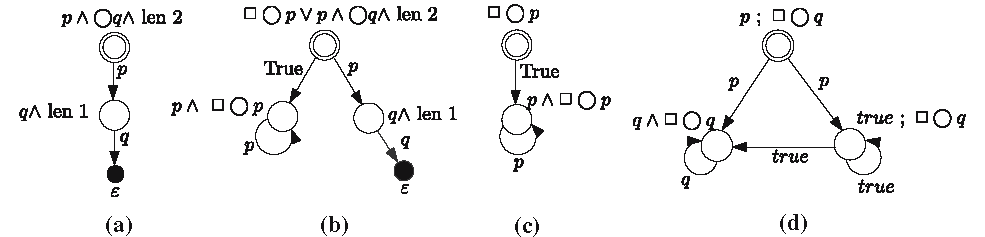
\includegraphics[width=1\textwidth]{NFG.png}
\end{figure}

  \item 带标签的范式图 \\
  由于 $prj$ 操作有明确的语义,$(P_1~,P_2)~prj~Q$ 的语义:
\begin{figure}[!h]
  \centering
  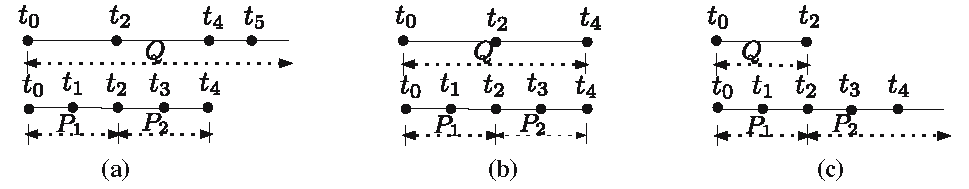
\includegraphics[width=1\textwidth]{prj.png}
\end{figure}

  即就是 PPTL 公式 $P_1$ 必须是有穷区间上的。但这一点在范式图上无法限制,所以加入标签。

\begin{figure}[!h]
  \centering
  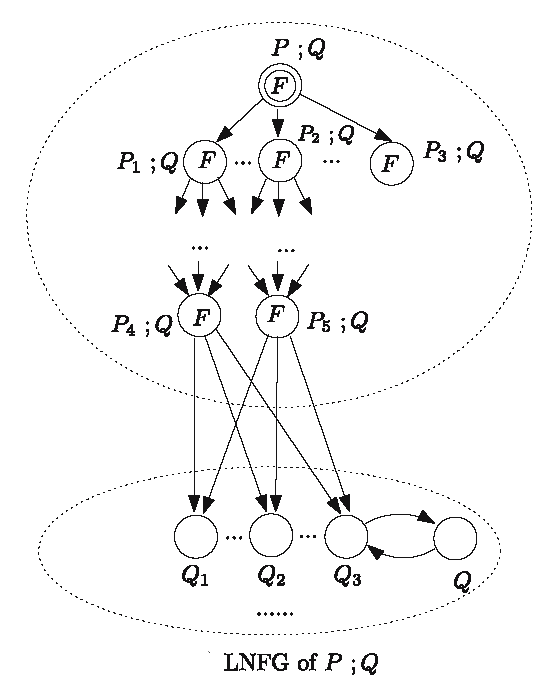
\includegraphics[width=0.6\textwidth]{LNFG.png}
\end{figure}
\end{enumerate}

\subsection{练习}

$\begin{array}{l}{\mathrm{NF}\left(\mathrm{O}^{2}(\square \bigcirc p ; q) \vee(p ; \square \bigcirc q)\right)} \\

\equiv \mathrm{NF}\left(\bigcirc^{2}(\square \bigcirc p ; q)\right) \vee \mathrm{NF}(p ; \square \bigcirc q) \\

\equiv \bigcirc(\bigcirc(\square \bigcirc p ; q)) \vee \operatorname{CHOP}(p ; \square \bigcirc q) \\

\equiv \bigcirc(\bigcirc(\square \bigcirc p ; q)) \vee \operatorname{CHOP}(\mathrm{NF}(p) ; \square \bigcirc q) \\

\equiv \bigcirc(\bigcirc(\square \bigcirc p ; q)) \vee \operatorname{CHOP}(p \wedge \varepsilon \vee p \wedge \text { Otrue; } \square \bigcirc q) \\

\equiv \bigcirc(\bigcirc(\square \bigcirc p ; q)) \vee \operatorname{CHOP}(p \wedge \varepsilon ; \square \bigcirc q) \vee \operatorname{CHOP}(p \wedge \text { Otrue; } \square \bigcirc q) \\

\equiv \bigcirc(\bigcirc(\square \bigcirc p ; q)) \vee p \wedge \operatorname{CHOP}(\varepsilon ; \square \bigcirc q) \vee p \wedge { \operatorname{CHOP}(\bigcirc true;} \square \bigcirc q ) \\

\equiv \bigcirc(\bigcirc(\square \bigcirc p ; q)) \vee p \wedge(\mathrm{NF}(\bigcirc q \wedge \varepsilon) \vee \mathrm{NF}(\bigcirc q \wedge \bigcirc \square \bigcirc q)) \vee p \wedge \bigcirc(\text {true} ; \square \bigcirc q) \\

{\equiv \bigcirc(\bigcirc(\square \bigcirc p ; q)) \vee p \wedge(f a l s e \vee \bigcirc(q \wedge \square \bigcirc q)) \vee p \wedge \bigcirc(\text {true} ; \square \bigcirc q)} \\ {\equiv \bigcirc(\bigcirc(\square \bigcirc p ; q)) \vee p \wedge \bigcirc(q \wedge \square \bigcirc q) \vee p \wedge \bigcirc(t r u e ; \square \bigcirc q)}
\end{array}$










